\date{}
\title{CSO2: Signals}
\date{}
\begin{document}

\begin{frame}{Agenda}
    \begin{itemize}
        \item Logistics
            \begin{itemize}

            \item \textbf{timing} homework due next Friday (uses signals)
            \item Week 04 quiz opens tonight
            \end{itemize}

        \item Last time: how do parent-child processes interact?
            \begin{itemize}
                \item waiting on processes
                \item file descriptors
            \end{itemize}

        \item This time:
            \begin{itemize}
                \item shell redirection
                \item pipes
                \item virtual memory
            \end{itemize}

    \end{itemize}
\end{frame}




\begin{frame}{last time: What happens when...}
\begin{itemize}
\item program runs an instruction the hardware can't complete?
    \begin{itemize}
    \item e.g. access memory it has not been allocated
    \item e.g. divide by zero
    \end{itemize}
\vspace{.5cm}
\item program asks the OS to do something?
    \begin{itemize}
    \item e.g. return process's \texttt{uid}
    \item e.g. wait for a key press (or other I/O operation)
    \end{itemize}
\vspace{.5cm}
\item<2> \textrightarrow hardware generates an \textit{exception}
\end{itemize}
\end{frame}


\begin{frame}{exceptions [Venn diagram]}
\begin{tikzpicture}
\node[very thick,draw,ellipse,blue,fill=blue!10,label={south:exceptions},minimum width=15cm,minimum height=6cm] (except) {};
\node[very thick,draw,circle,red,fill=red!10,label={[align=center]center:system\\calls},
      minimum width=3cm] (syscalls) 
    at ([xshift=-3cm,yshift=1cm]except.center){};
\node[very thick,draw,circle,red,fill=red!10,label={[align=center]center:faults\\\small (example:\\\small segfault)},
      minimum width=3cm] (fault) 
    at ([xshift=3cm,yshift=-1cm]except.center){};
\node[very thick,draw,circle,red,fill=red!10,label={[align=center]center:interrupts\\\small (example: I/O)},
      minimum width=3cm] (intr) 
    at ([xshift=0cm,yshift=0cm]except.center){};
\end{tikzpicture}
\end{frame}

\usetikzlibrary{decorations.pathreplacing}

\begin{frame}<0>[label=exceptTypesN]{types of exceptions}
\begin{itemize}
\item \tikzmark{int bot}\myemph<3>{externally-triggered}
    \begin{itemize}
    \item \myemph<3>{timer} --- keep program from hogging CPU
    \item \myemph<4>{I/O devices} --- key presses, hard drives, networks, \ldots
    \item \tikzmark{abort bot}hardware is broken (e.g. memory parity error)
    \end{itemize}
\item \tikzmark{trap bot}intentionally triggered exceptions
    \begin{itemize}
    \item \myemph<5>{system calls} --- ask OS to do something
    \end{itemize}
\item \tikzmark{fault bot}\myemph<6>{errors/events in programs}
    \begin{itemize}
        \item \myemph<7>{memory not in address space} (``Segmentation fault'')
        \item \myemph<8>{privileged instruction}
    \item divide by zero
    \item invalid instruction\tikzmark{invalid}
    \end{itemize}
\end{itemize}
\begin{tikzpicture}[overlay,remember picture]
    \coordinate (int top) at ([yshift=.6cm]pic cs:int bot);
    \coordinate (fault top) at ([yshift=.6cm]pic cs:fault bot);
    \coordinate (trap top) at ([yshift=.6cm]pic cs:trap bot);
    \coordinate (fault bot) at (pic cs:fault bot);
    \coordinate (over) at ([xshift=-4.5cm]current page.east);
    \coordinate (abort bot)  at (pic cs:abort bot);
    \coordinate (invalid bot)  at ([yshift=.6cm]pic cs:invalid bot);
    \draw[very thick,decorate,decoration={brace}] (int top -| over) -- (abort bot -| over) 
        node[midway,right,font=\large] (async label) {\myemph<2>{asynchronous}};
        \node[anchor=north west,font=\small,align=left] at ([xshift=.15cm,yshift=.3cm]async label.south west) {
            not triggered by \\
            running program
        };
    \draw[very thick,decorate,decoration={brace}] (trap top -| over) -- (invalid bot -| over) 
        node[midway,right,font=\large] (sync label) {\myemph<2>{synchronous}};
        \node[anchor=north west,font=\small,align=left] at ([xshift=.15cm,yshift=.3cm]sync label.south west) {
            triggered by \\
            current program
        };
\end{tikzpicture}
\end{frame}

\againframe<5>{exceptTypesN}

\section{not just timers}

\begin{frame}{I/O critical for today's computing}
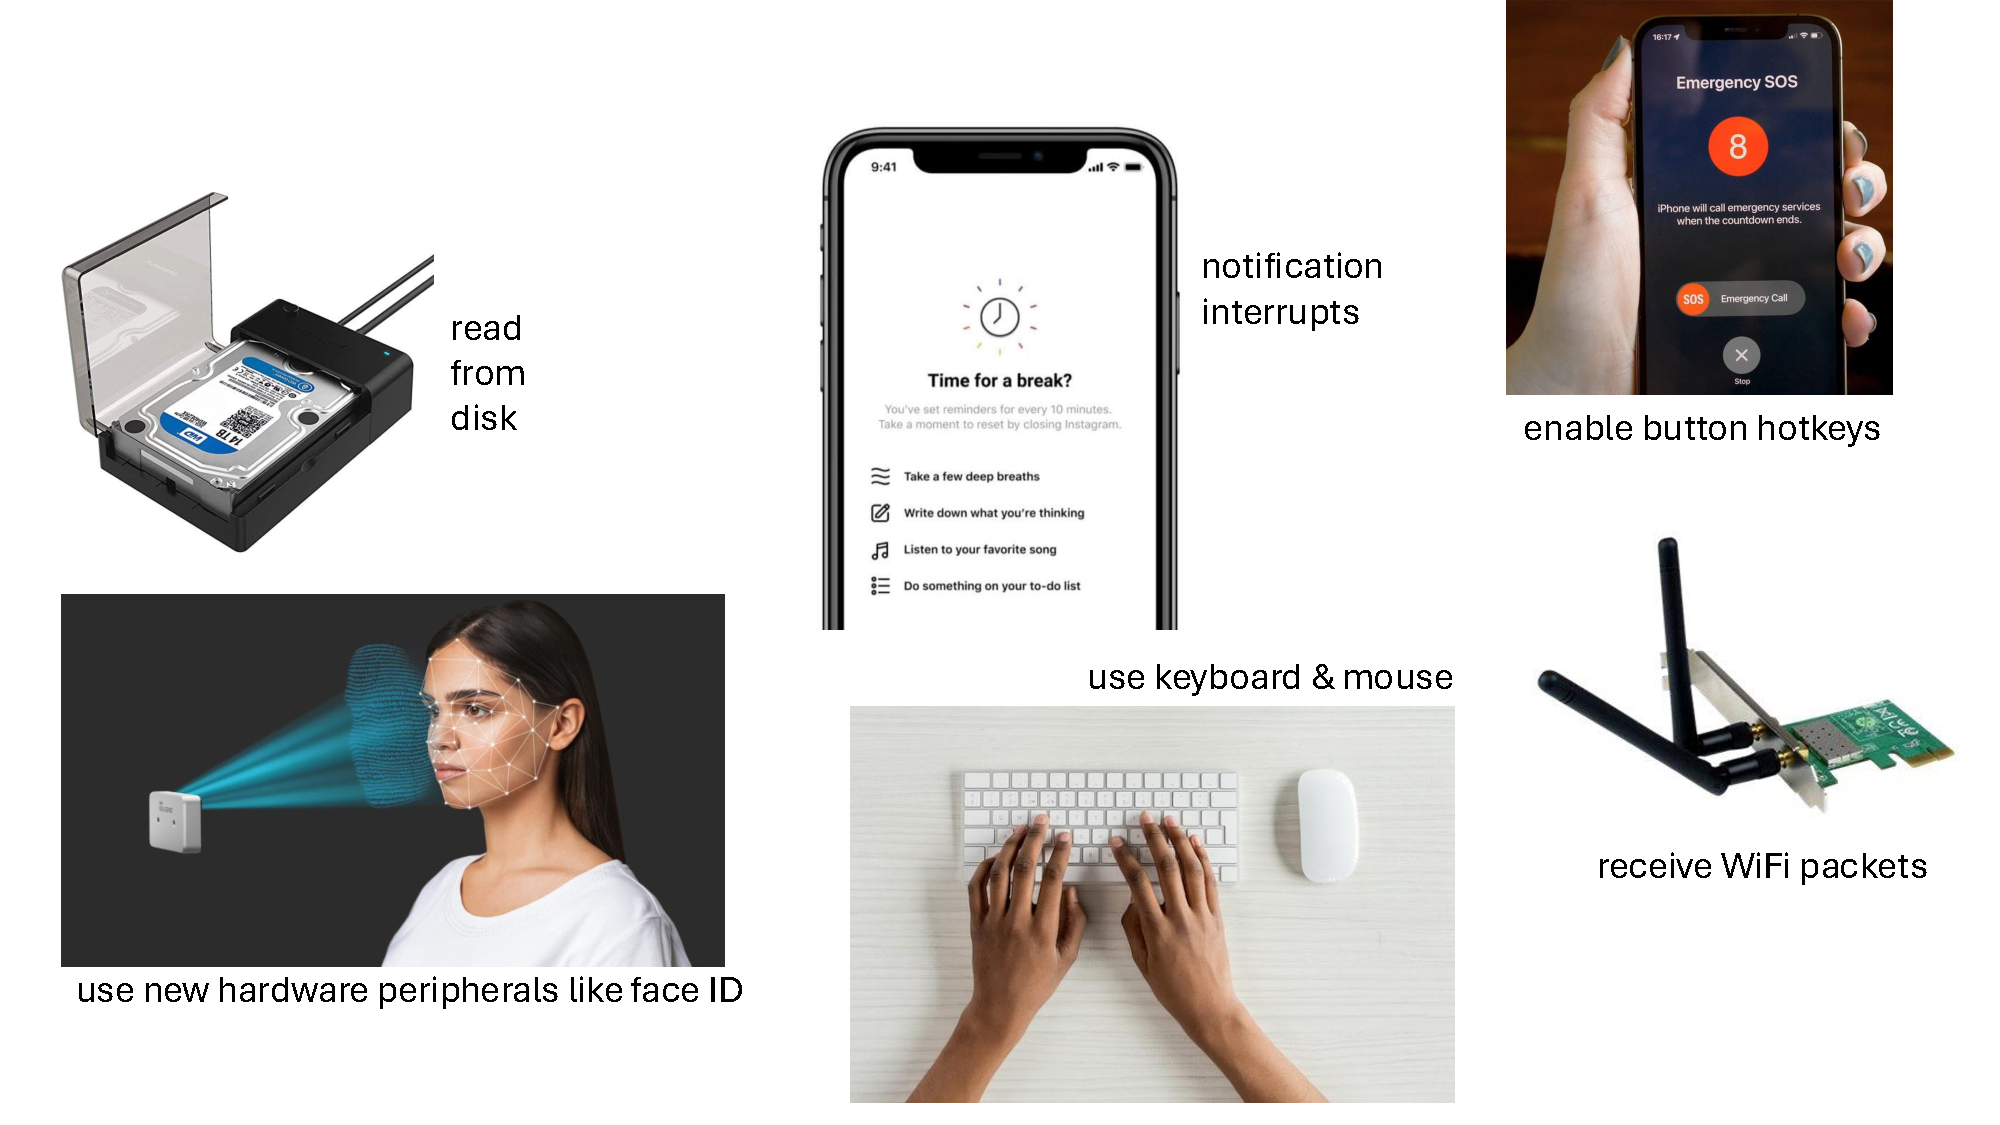
\includegraphics[width=0.9\pagewidth]{io.pdf}
\end{frame}

\subsection{typical I/O pattern}
\begin{frame}{exception patterns with I/O (1)}
    \begin{itemize}
    \item input --- available now:
        \begin{itemize}
        \item exception: device says ``I have input now''
        \item handler: OS stores input for later
        \item exception (syscall): program says ``I want to read input''
        \item handler: OS returns that input
        \end{itemize}
    \item input --- not available now:
        \begin{itemize}
        \item exception (syscall): program says ``I want to read input''
        \item handler: OS runs other things (context switch)
        \item exception: device says ``I have input now''
        \item handler: OS retrieves input
        \item handler: (possibly) OS switches back to program that wanted it
        \end{itemize}
    \end{itemize}
\end{frame}

\begin{frame}{exception patterns with I/O (2)}
    \begin{itemize}
    \item output --- ready now:
        \begin{itemize}
        \item exception (syscall): program says ``I want to output this'
        \item handler: OS sends output to device
        \end{itemize}
    \item output --- not ready now
        \begin{itemize}
        \item exception (syscall): program says ``I want to output''
        \item handler: OS realizes device can't accept output yet
        \item (other things happen)
        \item exception: device says ``I'm ready for output now''
        \item handler: OS sends output requested earlier
        \end{itemize}
    \end{itemize}
\end{frame}


\usetikzlibrary{patterns}

\begin{frame}{keyboard input timeline}
\begin{tikzpicture}
\tikzset{
    prog1/.style={draw,fill=cyan},
    prog2/.style={draw,fill=green},
    prog3/.style={draw,fill=violet!30},
    proglabel/.style={font=\tt\scriptsize},
    labelprog1/.style={execute at begin node={\strut },pin={south:\tt\scriptsize read\_input.exe}},
    labelprog2/.style={execute at begin node={\strut }},
    labelprog3/.style={execute at begin node={\strut }},
}
\begin{scope}[xscale=1.5,yscale=1]
\foreach \s/\e/\p [count=\x] in {0/0.5/1,0.5/3/2,3/5.4/3,5.4/7/1} {
    \coordinate (s-\x) at (\s, 0);
    \coordinate (e-\x) at (\e, 0);
    \draw[prog\p] (\s, 0) rectangle (\e, 1) coordinate[midway] (mid-\x);
    \node[anchor=center,proglabel,labelprog\p] at (mid-\x) {};
    \begin{pgfonlayer}{fg}
    \draw[fill=white] ([xshift=-.05cm]e-\x) rectangle ([xshift=.05cm,yshift=1cm]e-\x);
    \draw[pattern=north west lines] ([xshift=-.05cm]e-\x) rectangle ([xshift=.05cm,yshift=1cm]e-\x);
    \end{pgfonlayer}
}
\end{scope}
% FIXME: mark types of exceptions at each transition
\draw[red,very thick,Latex-] ([xshift=-.05cm]e-1) -- (2, -3) node[fill=white,draw] {trap --- {\tt read} system call};
\draw[red,very thick,Latex-] ([xshift=-.05cm]e-3) -- (7, -4) node[fill=white,draw] {interrupt --- from keyboard};
\begin{scope}[xshift=2cm]
\draw[fill=white,pattern=north west lines] (0, -1) rectangle (1, -2);
\node[anchor=west] at (1, -1.5) {\strut = operating system};
\end{scope}
\end{tikzpicture}
\end{frame}




\section{review: exception / context switch}
\begin{frame}{review: definitions}
\begin{itemize}
\item exception: hardware calls OS specified routine
    \begin{itemize}
    \item many possible reasons
    \item system calls: type of exception
    \end{itemize}
\item context switch: OS switches to another thread
    \begin{itemize}
    \item by saving old register values + loading new ones
    \item part of OS routine run by exception
    \end{itemize}
\end{itemize}
\end{frame}


\section{exercise}
\begin{frame}{which of these require exceptions? context switches?}
    \begin{itemize}
    \item A. program calls a function in the standard library
    \item B. program writes a file to disk
    \item C. program A goes to sleep, letting program B run
    \item D. program exits
    \item E. program returns from one function to another function
    \item F. program pops a value from the stack
    \end{itemize}
\end{frame}

\iftoggle{heldback}{}{
\begin{frame}{which require exceptions [answers] (1)}
\begin{itemize}
    \item A. program calls a function in the standard library
        \begin{itemize}
        \item no (same as other functions in program; some standard library functions might make system calls, but if so, that'll be part of what happens after they're called and before they return)
        \end{itemize}
    \item B. program writes a file to disk
        \begin{itemize}
        \item yes (requires kernel mode only operations)
        \end{itemize}
    \item C. program A goes to sleep, letting program B run
        \begin{itemize}
        \item yes (kernel mode usually required to change the address space to acess program B's memory)
        \end{itemize}
\end{itemize}
\end{frame}
\begin{frame}{which require exceptions [answer] (2)}
    \begin{itemize}
    \item D. program exits
        \begin{itemize}
        \item yes (requires switching to another program, which requires accessing OS data + other program's memory)
        \end{itemize}
    \item E. program returns from one function to another function
        \begin{itemize}
        \item no
        \end{itemize}
    \item F. program pops a value from the stack
        \begin{itemize}
        \item no
        \end{itemize}
    \end{itemize}
\end{frame}

\begin{frame}{which require context switches [answer]}
    \begin{itemize}
    \item no: A. program calls a function in the standard library
    \item no: B. program writes a file to disk
        \begin{itemize}
        \item (but might be done if program needs to wait for disk and other things could be run while it does)
        \end{itemize}
    \item yes: C. program A goes to sleep, letting program B run
    \item yes: D. program exits
    \item no: E. program returns from one function to another function
    \item no: F. program pops a value from the stack
    \end{itemize}
\end{frame}
}


\subsection{aside: terms}
\begin{frame}{terms for exceptions}
    \begin{itemize}
    \item terms for exceptions aren't standardized
    \vspace{.5cm}
    \item our readings use one set of terms
    \begin{itemize}
        \item interrupts = externally-triggered
        \item faults = error/event in program
        \item trap = intentionally triggered
        \end{itemize}
    \item all these terms appear differently elsewhere
    \end{itemize}
\end{frame}


\section{process}
\begin{frame}{The Process}
\begin{itemize}
\item \myemph{process} = thread(s) + address space
\item illusion of \myemph{dedicated machine}:
\begin{itemize}
\item thread = illusion of own CPU
\item address space = illusion of own memory
\end{itemize}
\end{itemize}
\end{frame}









\begin{frame}
    \titlepage
\end{frame}



\makeatletter
\newenvironment<>{btHighlight}[1][]
{\begin{onlyenv}#2\begingroup\tikzset{bt@Highlight@par/.style={#1}}\begin{lrbox}{\@tempboxa}}
{\end{lrbox}\bt@HL@box[bt@Highlight@par]{\@tempboxa}\endgroup\end{onlyenv}}

\newcommand<>\btHL[1][]{%
  \only#2{\begin{btHighlight}[#1]\bgroup\aftergroup\bt@HL@endenv}%
}
\def\bt@HL@endenv{%
  \end{btHighlight}%   
  \egroup %
}
\tikzset{
    btHLbox/.style={
        fill=red!30,outer sep=0pt,inner xsep=1pt, inner ysep=0pt, rounded corners=3pt
    },
}
\newcommand{\bt@HL@box}[2][]{%
  \tikz[#1]{%
    \pgfpathrectangle{\pgfpoint{1pt}{0pt}}{\pgfpoint{\wd #2}{\ht #2}}%
    \pgfusepath{use as bounding box}%
    \node[text width={},draw=none,anchor=base west, btHLbox, minimum height=\ht\strutbox+1pt,#1]{\raisebox{1pt}{\strut}\strut\usebox{#2}};
  }%
}

\lst@CCPutMacro
    \lst@ProcessOther {"2A}{%
      \lst@ttfamily 
         {\raisebox{2pt}{*}}% used with ttfamily
         {\raisebox{2pt}{*}}}% used with other fonts
    \@empty\z@\@empty

\lstdefinelanguage
   [x8664gas]{Assembler}     % add a "x64" dialect of Assembler
   [x86masm]{Assembler} % based on the "x86masm" dialect
   % with these extra keywords:
   {morekeywords={CDQE,CQO,CMPSQ,CMPXCHG16B,JRCXZ,LODSQ,MOVSXD,%
                  POPFQ,PUSHFQ,SCASQ,STOSQ,IRETQ,RDTSCP,SWAPGS,.TEXT,.STRING,.ASCIZ,%
                  BEQ,LW,SW,LB,SB,ADDIU,J,BEQZ,BNEZ,BNE,%
                  MOVUPD,MULPD,MOVSD,MULSD,%
                  SHLADD,MOV,CMP.LT,TBIT.NZ,BR.RET.SPTK.MANY,%
                  ADDQ,POPQ,PUSHQ,RRMOVQ,MRMOVQ,RMMOVQ,IRMOVQ,%
                  <-,LL,SC,ADDI,ADDL,VMOVDQA,ADDQ,CMPL,JB,JBE,MOVL,CLTQ,
                  MOVW,PUSHW,MOV,ADD,SUB,INT,PUSH,MOV,ADD,REP,MOVSB,%
                  TESTQ,CMPQ,MOVL,MOVQ,ADDQ,JMPQ,XORQ,%
                  LEAQ,LEAL,LEA,RETQ,RET,POPL,POPW,PUSHL,PUSHW,%
                  LEAW,%
                  SUBQ,SYSCALL,.ASCII,CALLQ,MOVSLQ,JMP,ANDQ,SHRQ,MOVB,INCQ,TESTL,XORL,%
                  SHRL,LEAL,SARL,SUBL,IMULL,IMULQ,MOVDQU,PADDD,XORL,%
                  MOVZBL,MOVZB,SHRB,SRAL,SHRL,ANDL,%
                  CMOVNS,SRAL,SRAQ,MOVZBW,MOVZBQ,%
                  PADDW,PADDQ,MODUPS,MOVAPD,%
                  MOVL,RET,.GLOBL,%
                  },
    deletekeywords={eax,ebx,sp,si,cx,di,ds,cs,es,fs,dx,ax,bx,al,esi,ebp,ecx,rip,eip,edx,edi,rdi,esp},
    morecomment=[l]{\#},
    morecomment=[l]{\/\/},
    morecomment=[s]{/*}{*/},
    sensitive=false,
    keepspaces=true} % et

\lstalias[]{myasm}[x8664gas]{Assembler}

\lstdefinelanguage{JavaScript}{
  keywords={typeof, new, true, false, catch, function, return, null, catch, switch, var, if, in, while, do, else, case, break},
  ndkeywords={class, export, boolean, throw, implements, import, this},
  sensitive=false,
  comment=[l]{//},
  morecomment=[s]{/*}{*/},
  morestring=[b]',
  morestring=[b]"
}

\newcommand{\keywordstyle}{\sourcecodeprolight\bfseries\color{blue!30!black}}
\newcommand{\stringstyle}{\color{blue!20!black}\ttfamily}

\lstset{
    language=C,
    basicstyle=\sourcecodepro\EmptyMapping,
    escapechar=`,
    keywordstyle=\keywordstyle\EmptyMapping,
    identifierstyle=\sourcecodepro\EmptyMapping,
    numberstyle=\small\color{black!70},
    commentstyle=\color{red!60!black}\ttfamily\itshape,
    stringstyle=\color{blue!20!black}\ttfamily,
    ndkeywordstyle=\bfseries\color{blue!30!black},
    upquote=true,
}



\lstdefinestyle{medium}{
    basicstyle=\sourcecodepro\EmptyMapping\fontsize{12}{13}\selectfont,
    keywordstyle=\sourcecodepro\EmptyMapping\fontsize{12}{13}\selectfont\keywordstyle,
}

\lstdefinestyle{small}{
    basicstyle=\sourcecodepro\EmptyMapping\small,
    keywordstyle=\sourcecodepro\EmptyMapping\small\keywordstyle,
}

\lstdefinestyle{smaller}{
    basicstyle=\sourcecodepro\EmptyMapping\fontsize{11}{12}\selectfont,
    keywordstyle=\sourcecodepro\EmptyMapping\fontsize{11}{12}\selectfont\keywordstyle,
}


\lstdefinestyle{script}{
    basicstyle=\sourcecodepro\EmptyMapping\scriptsize,
    keywordstyle=\sourcecodepro\EmptyMapping\scriptsize\bfseries,
}





\makeatletter
\newenvironment<>{btHighlight}[1][]
{\begin{onlyenv}#2\begingroup\tikzset{bt@Highlight@par/.style={#1}}\begin{lrbox}{\@tempboxa}}
{\end{lrbox}\bt@HL@box[bt@Highlight@par]{\@tempboxa}\endgroup\end{onlyenv}}

\newcommand<>\btHL[1][]{%
  \only#2{\begin{btHighlight}[#1]\bgroup\aftergroup\bt@HL@endenv}%
}
\def\bt@HL@endenv{%
  \end{btHighlight}%   
  \egroup %
}
\tikzset{
    btHLbox/.style={
        fill=red!30,outer sep=0pt,inner xsep=1pt, inner ysep=0pt, rounded corners=3pt
    },
}
\newcommand{\bt@HL@box}[2][]{%
  \tikz[#1]{%
    \pgfpathrectangle{\pgfpoint{1pt}{0pt}}{\pgfpoint{\wd #2}{\ht #2}}%
    \pgfusepath{use as bounding box}%
    \node[text width={},draw=none,anchor=base west, btHLbox, minimum height=\ht\strutbox+1pt,#1]{\raisebox{1pt}{\strut}\strut\usebox{#2}};
  }%
}

\lst@CCPutMacro
    \lst@ProcessOther {"2A}{%
      \lst@ttfamily 
         {\raisebox{2pt}{*}}% used with ttfamily
         {\raisebox{2pt}{*}}}% used with other fonts
    \@empty\z@\@empty

\lstdefinelanguage
   [x8664gas]{Assembler}     % add a "x64" dialect of Assembler
   [x86masm]{Assembler} % based on the "x86masm" dialect
   % with these extra keywords:
   {morekeywords={CDQE,CQO,CMPSQ,CMPXCHG16B,JRCXZ,LODSQ,MOVSXD,%
                  POPFQ,PUSHFQ,SCASQ,STOSQ,IRETQ,RDTSCP,SWAPGS,.TEXT,.STRING,.ASCIZ,%
                  BEQ,LW,SW,LB,SB,ADDIU,J,BEQZ,BNEZ,BNE,%
                  MOVUPD,MULPD,MOVSD,MULSD,%
                  SHLADD,MOV,CMP.LT,TBIT.NZ,BR.RET.SPTK.MANY,%
                  ADDQ,POPQ,PUSHQ,RRMOVQ,MRMOVQ,RMMOVQ,IRMOVQ,%
                  <-,LL,SC,ADDI,ADDL,VMOVDQA,ADDQ,CMPL,JB,JBE,MOVL,CLTQ,
                  MOVW,PUSHW,MOV,ADD,SUB,INT,PUSH,MOV,ADD,REP,MOVSB,%
                  TESTQ,CMPQ,MOVL,MOVQ,ADDQ,JMPQ,XORQ,%
                  LEAQ,LEAL,LEA,RETQ,RET,POPL,POPW,PUSHL,PUSHW,%
                  LEAW,%
                  SUBQ,SYSCALL,.ASCII,CALLQ,MOVSLQ,JMP,ANDQ,SHRQ,MOVB,INCQ,TESTL,XORL,%
                  SHRL,LEAL,SARL,SUBL,IMULL,IMULQ,MOVDQU,PADDD,XORL,%
                  MOVZBL,MOVZB,SHRB,SRAL,SHRL,ANDL,%
                  CMOVNS,SRAL,SRAQ,MOVZBW,MOVZBQ,%
                  PADDW,PADDQ,MODUPS,MOVAPD,%
                  MOVL,RET,.GLOBL,%
                  },
    deletekeywords={eax,ebx,sp,si,cx,di,ds,cs,es,fs,dx,ax,bx,al,esi,ebp,ecx,rip,eip,edx,edi,rdi,esp},
    morecomment=[l]{\#},
    morecomment=[l]{\/\/},
    morecomment=[s]{/*}{*/},
    sensitive=false,
    keepspaces=true} % et

\lstalias[]{myasm}[x8664gas]{Assembler}

\lstdefinelanguage{JavaScript}{
  keywords={typeof, new, true, false, catch, function, return, null, catch, switch, var, if, in, while, do, else, case, break},
  ndkeywords={class, export, boolean, throw, implements, import, this},
  sensitive=false,
  comment=[l]{//},
  morecomment=[s]{/*}{*/},
  morestring=[b]',
  morestring=[b]"
}

\newcommand{\keywordstyle}{\sourcecodeprolight\bfseries\color{blue!30!black}}
\newcommand{\stringstyle}{\color{blue!20!black}\ttfamily}

\lstset{
    language=C,
    basicstyle=\sourcecodepro\EmptyMapping,
    escapechar=`,
    keywordstyle=\keywordstyle\EmptyMapping,
    identifierstyle=\sourcecodepro\EmptyMapping,
    numberstyle=\small\color{black!70},
    commentstyle=\color{red!60!black}\ttfamily\itshape,
    stringstyle=\color{blue!20!black}\ttfamily,
    ndkeywordstyle=\bfseries\color{blue!30!black},
    upquote=true,
}



\lstdefinestyle{medium}{
    basicstyle=\sourcecodepro\EmptyMapping\fontsize{12}{13}\selectfont,
    keywordstyle=\sourcecodepro\EmptyMapping\fontsize{12}{13}\selectfont\keywordstyle,
}

\lstdefinestyle{small}{
    basicstyle=\sourcecodepro\EmptyMapping\small,
    keywordstyle=\sourcecodepro\EmptyMapping\small\keywordstyle,
}

\lstdefinestyle{smaller}{
    basicstyle=\sourcecodepro\EmptyMapping\fontsize{11}{12}\selectfont,
    keywordstyle=\sourcecodepro\EmptyMapping\fontsize{11}{12}\selectfont\keywordstyle,
}


\lstdefinestyle{script}{
    basicstyle=\sourcecodepro\EmptyMapping\scriptsize,
    keywordstyle=\sourcecodepro\EmptyMapping\scriptsize\bfseries,
}




\section{signals}

\subsection{idea}

\usetikzlibrary{shapes.callouts,positioning}

\begin{frame}{signals}
\begin{itemize}
\item Unix-like \myemph{operating system feature}
\item like exceptions for processes:
\vspace{.5cm}
\item can be triggered by external process
    \begin{itemize}
    \item kill command/system call
    \end{itemize}
\item can be triggered by special events
    \begin{itemize}
    \item pressing control-C
    \item other events that would normal terminate program
        \begin{itemize}
        \item `segmentation fault'
        \item illegal instruction
        \item divide by zero
        \end{itemize}
    \end{itemize}
\item can invoke \myemph{signal handler} (like exception handler)
\end{itemize}
\end{frame}

\begin{frame}{exceptions v signals}

\begin{tabular}{l|l}
(hardware) exceptions & signals \\ \hline
handler runs in kernel mode & handler runs in user mode \\
hardware decides when & \myemph<2>{OS decides}~\tikzmark{OS when}\myemph<2>{when} \\
hardware needs to save PC & OS needs to save PC \tikzmark{plus regs}\myemph<3>{+ registers} \\
\myemph<4>{processor} program counter changes& \myemph<4>{thr\tikzmark{thread}ead} program counter changes \\
\end{tabular}
{\small program counter = instruction to run next}
\begin{tikzpicture}[overlay,remember picture]
\coordinate (callout mark) at ([xshift=-2cm,yshift=-2cm]pic cs:OS when);
\begin{visibleenv}<2>
    \node[align=left,my callout=OS when,anchor=north] at (callout mark) {
        \ldots but OS needs to run to trigger handler \\
        most  likely ``forwarding'' hardware exception
    };
\end{visibleenv}
\begin{visibleenv}<3>
    \node[align=left,my callout=plus regs,anchor=north] at (callout mark) {
        signal handler follows normal calling convention \\
        not special assembly like typical exception handler
    };
\end{visibleenv}
\begin{visibleenv}<4>
    \node[align=left,my callout=thread,anchor=north] at (callout mark) {
        signal handler runs in same thread (`virtual processor') \\
        as process was using before \\
        ~ \\
        not running at `same time' as the code it interrupts
    };
\end{visibleenv}
\end{tikzpicture}
\end{frame}



\subsection{example / sigaction}

\begin{frame}{signal API}
\begin{itemize}
    \item {\tt sigaction} --- register handler for signal
    \item {\tt kill} --- send signal to process
    \item {\tt pause} --- put process to sleep until signal received
    \item {\tt sigprocmask} --- temporarily block some signals from being received
    \item \ldots{} and much more
\end{itemize}
\end{frame}

\begin{frame}[fragile,label=exSignals]{example signal program}
\lstset{
    language=C,
    basicstyle={\tt\fontsize{10.5}{11}\selectfont},
    moredelim=**[is][\btHL<1|handout:1>]{@1}{@},
    moredelim=**[is][\btHL<2|handout:2>]{@2}{@},
    moredelim=**[is][\btHL<3|handout:3>]{@3}{@},
    moredelim=**[is][\btHL<4|handout:4>]{@4}{@},
}
\lstinputlisting{sigex.c}
\end{frame}



\subsection{signal IDs/events}

\begin{frame}{SIGxxxx}
\begin{itemize}
\item signals types identified by number\ldots
\item constants declared in \texttt{<signal.h>}
\end{itemize}
\small
\begin{tabular}{l|l}
constant & likely use \\\hline
SIGBUS & ``bus error''; certain types of invalid memory accesses \\
SIGSEGV & ``segmentation fault''; other types of invalid memory accesses \\
SIGINT & what control-C usually does \\
SIGFPE & ``floating point exception''; includes integer divide-by-zero \\
SIGHUP, SIGPIPE & reading from/writing to disconnected terminal/socket \\
SIGUSR1, SIGUSR2 & use for whatever you (app developer) wants \\
SIGKILL & terminates process \myemph<2>{(cannot be handled by process!)} \\
SIGSTOP & suspends process \myemph<2>{(cannot be handled by process!)} \\
\ldots & \ldots \\
\end{tabular}
\end{frame}


% FIXME: handling SIGSEGV???

\subsection{wait, SIGSEGV?}

\begin{frame}[fragile,label=handleSIGSEGV]{handling Segmentation Fault}
\lstset{language=C,style=smaller}
\begin{lstlisting}
...
void handle_sigsegv(int num) {
    puts("got SIGSEGV");
}

int main(void) {
    struct sigaction act;
    act.sa_handler = handle_sigsegv;
    sigemptyset(&act.sa_mask);
    act.sa_flags = 0;
    sigaction(SIGSEGV, &act, NULL);

    asm("movq %rax, 0x12345678");
}
\end{lstlisting}
\hrule
\begin{visibleenv}<2->
\begin{Verbatim}
got SIGSEGV
got SIGSEGV
got SIGSEGV
got SIGSEGV
got SIGSEGV
got SIGSEGV
got SIGSEGV
got SIGSEGV
got SIGSEGV
got SIGSEGV
got SIGSEGV
got SIGSEGV
\end{Verbatim}
\end{visibleenv}
\end{frame}


\subsection{signal API}


\begin{frame}{signal API}
\begin{itemize}
    \item {\tt sigaction} --- register handler for signal
    \item {\tt kill} --- send signal to process
    \item {\tt pause} --- put process to sleep until signal received
    \item {\tt sigprocmask} --- temporarily block some signals from being received
    \item \ldots{} and much more
\end{itemize}
\end{frame}


% FIXME: proecss ID stuff?

\subsection{exercise}
\begin{frame}[fragile,label=signalEx]{output of this?}
\lstset{language=C,style=script}
\begin{tikzpicture}
\node[draw,very thick,label={north:pid 1000}] (left) {
\begin{lstlisting}
void handle_usr1(int num) {
    write(1, "X", 1);
    kill(2000, SIGUSR1);
    _exit(0);
}
int main() {
    struct sigaction act; 
    ... // initialize rest of "act"
    act.sa_handler = &handle_usr1;
    sigaction(SIGUSR1, &act, NULL);
    kill(1000, SIGUSR1);
}
\end{lstlisting}
};
\node[anchor=north west,draw,very thick,label={north:pid 2000}] (right) at ([xshift=1cm]left.north east) {
\begin{lstlisting}
void handle_usr1(int num) {
    write(1, "Y", 1);
    _exit(0);
}
int main() {
    struct sigaction act;
    ... // initialize rest of "act"
    act.sa_handler = &handle_usr1;
    sigaction(SIGUSR1, &act, NULL);
}
\end{lstlisting}
};
\end{tikzpicture}

If these run at same time, expected output?
\begin{tabular}{lll}
A. XY & B. X & C. Y \\
D. YX & E. X or XY, depending on timing & F. crash \\
G. (nothing) & H. something else \\
\end{tabular}
\end{frame}

\begin{frame}[fragile,label=signalEx2]{output of this? (v2)}
\vspace{-0.1cm}
\lstset{
    language=C,
    style=script,
    moredelim=**[is][\btHL<1|handout:1>]{@1}{@},
}
\begin{tikzpicture}
    \node[draw,very thick,label={[inner sep=0mm]north:pid 1000}] (left) {
\begin{lstlisting}
void handle_usr1(int num) {
    write(1, "X", 1);
    kill(2000, SIGUSR1);
    _exit(0);
}
int main() {
    struct sigaction act;
    ... // initialize rest of "act"
    act.sa_handler = &handle_usr1;
    sigaction(SIGUSR1, &act);
    @1sleep(1);@
    kill(1000, SIGUSR1);
    @1while (1) pause();@
}
\end{lstlisting}
};
\node[anchor=north west,draw,very thick,label={[inner sep=0mm]north:pid 2000}] (right) at ([xshift=1cm]left.north east) {
\begin{lstlisting}
void handle_usr1(int num) {
    write(1, "Y", 1);
    _exit(0);
}
int main() {
    struct sigaction act;
    ... // initialize rest of "act"
    act.sa_handler = &handle_usr1;
    sigaction(SIGUSR1, &act);
    @1while (1) pause();@
}
\end{lstlisting}
};
\end{tikzpicture}
\vspace{-0.1cm}

If these run at same time, expected output?
\begin{tabular}{lll}
A. XY & B. X & C. Y \\
D. YX & E. X or XY, depending on timing & F. crash \\
G. (nothing) & H. something else \\
\end{tabular}
\end{frame}


\subsection{delivery}

\usetikzlibrary{arrows.meta,matrix}
\begin{frame}{x86-64 Linux signal delivery (1)}
\begin{itemize}
\item suppose: signal happens while {\tt foo()} is running
\item OS saves registers \myemph{to user stack}
\item OS modifies user registers, PC to call signal handler
\end{itemize}
\begin{tikzpicture}
\tikzset{every node/.style={font=\small}}
\matrix[tight matrix,nodes={text width=6cm},label={the stack}] (stack) {
    address of {\tt \_\_restore\_rt} \\
    saved registers \\
    PC when signal happened \\
    local variables for foo \\
    \ldots{} \\
};
\draw[thick,-Latex] (stack-4-1.east) -- ++(.5cm,0cm) node[right,align=left] {stack pointer \\ before signal delivered};
\draw[thick,-Latex] (stack-1-1.east) -- ++(.5cm,0cm) node[right,align=left] {stack pointer \\ when signal handler started};
\end{tikzpicture}
\end{frame}

\begin{frame}[fragile,label=sigReturn]{x86-64 Linux signal delivery (2)}
\lstset{
    language=myasm,
    style=small,
    morekeywords={ret,syscall,movq}
}
\begin{lstlisting}
handle_sigint:
    ...
    ret
...
__restore_rt:
    // 15 = "sigreturn" system call
    movq $15, %rax
    syscall
\end{lstlisting}
\begin{itemize}
\item {\tt \_\_restore\_rt} is \myemph{return address} for signal handler
\item sigreturn syscall restores pre-signal state
\begin{itemize}
    \item if SA\_RESTART set, restarts interrupted operation
    \item also handles caller-saved registers
    \item also might change which signals blocked (depending how sigaction was called)
\end{itemize}
\end{itemize}
\end{frame}




\subsection{caution: signal-safety}

\usetikzlibrary{arrows.meta}

\begin{frame}{signal handler unsafety (0)}
\lstset{
    language=C,
    style=small,
    moredelim=**[is][\btHL<2|handout:2>]{@2}{@},
}
\lstinputlisting{../signals/unsafe-signal-0.c}
\end{frame}

\begin{frame}{signal handler unsafety (1)}
\lstset{
    language=C,
    style=smaller,
    moredelim=**[is][\btHL<2|handout:2>]{@1}{@},
    moredelim=**[is][\btHL<2|handout:2>]{@2}{@},
}
\lstinputlisting{../signals/unsafe-signal.c}
\end{frame}

\begin{frame}{signal handler unsafety (2)}
\lstset{
    language=C,
    style=smaller,
    moredelim=**[is][\btHL<1|handout:1>]{@1}{@},
    moredelim=**[is][\btHL<2|handout:2>]{@2}{@},
}
\lstinputlisting{../signals/unsafe-signal-2.c}
\end{frame}

\begin{frame}[fragile,label=unsafeTime]{signal handler unsafety: timeline}
\begin{tikzpicture}
\tikzset{every node/.style={font=\small},>=Latex,myline/.style={very thick}}
\node[draw] (fooStart) {
foo starts
};
\node[draw,anchor=north west] (mallocStart) at ([yshift=-.25cm,xshift=1cm]fooStart.south west) {
    malloc: \lstinline|to_return = next_to_return;|
};
\draw[->,myline] ([xshift=.5cm]fooStart.south west) |- (mallocStart.west);
\node[draw,anchor=north west] (sigintStart) at ([yshift=-.25cm,xshift=1cm]mallocStart.south west) {
    handle\_sigint
};
\draw[->,myline] ([xshift=.5cm]mallocStart.south west) |- (sigintStart.west);
\node[draw,anchor=north west] (printfStart) at ([yshift=-.25cm,xshift=1cm]sigintStart.south west) {
    printf
};
\draw[->,myline] ([xshift=.5cm]sigintStart.south west) |- (printfStart.west);
\node[draw,anchor=north west,align=left] (mallocStart2) at ([yshift=-.25cm,xshift=1cm]printfStart.south west) {
    malloc: \lstinline|to_return = next_to_return;| \\
    malloc: \lstinline|next_to_return += ...;| \\
};
\draw[->,myline] ([xshift=.5cm]printfStart.south west) |- (mallocStart2.west);
\node[draw,anchor=north west,align=left] (printfDone) at ([yshift=-.25cm,xshift=-1cm]mallocStart2.south west) {
    printf: store/use returned {\tt buf}
};
\draw[->,myline] ([xshift=.5cm]printfStart.south west) -- ([xshift=.5cm]printfDone.north west);
\node[draw,anchor=north west,align=left] (fooFinish) at ([yshift=-.25cm,xshift=-3cm]printfDone.south west) {
    foo: \myemph{malloc returns pointer {\tt printf} is using!}
};
\draw[->,myline] ([xshift=.5cm]fooStart.south west) -- ([xshift=.5cm]fooFinish.north west);
\end{tikzpicture}
\end{frame}

\begin{frame}{signal handler unsafety (3)}
\lstset{
    language=C,
    basicstyle={\tt\fontsize{10}{11}\selectfont},
    moredelim=**[is][\btHL<1|handout:1>]{@1}{@},
    moredelim=**[is][\btHL<2|handout:2>]{@2}{@},
}
\lstinputlisting{../signals/unsafe-signal-3.c}
\end{frame}

\begin{frame}{signal handler safety}
\begin{itemize}
\item POSIX (standard that Linux follows) defines ``async-signal-safe'' functions
    \begin{itemize}
    \item \texttt{man signal-safety} can get you list on portal
    \end{itemize}
\item these must work correctly no matter what they interrupt
\item \ldots and no matter how they are interrupted
\item includes: {\tt write}, {\tt \_exit}
\item does not include: {\tt printf}, {\tt malloc}, {\tt exit}
\end{itemize}
\end{frame}




\subsection{alt signal handling}

\usetikzlibrary{arrows.meta,decorations.pathmorphing,decorations.pathreplacing}
\begin{frame}{blocking signals}
\begin{itemize}
\item avoid having signal handlers anywhere:
\item can instead \myemph{block signals}
    \begin{itemize}
    \item \texttt{sigprocmask()}, \texttt{pthread\_sigmask()}
    \end{itemize}
\item blocked = signal handler doesn't run
    \begin{itemize}
    \item also called ``masking'' a signal
    \item blocked signals are not \textit{delivered} (acted on)
    \end{itemize}
\item instead, signal becomes \textit{pending}
    \begin{itemize}
    \item delivered if unblocked
    \end{itemize}
\end{itemize}
\begin{tikzpicture}[overlay,remember picture]
\begin{visibleenv}<2->
\coordinate (base) at ([xshift=-2cm,yshift=-1cm]current page.north east);
\draw[very thick,decoration={snake},decorate,-Latex] (base) -- ++(0cm, -8cm) coordinate (snake bottom);
\draw[thick,dotted] ([yshift=-.5cm]base) -- ++(-.5cm,0cm) node[font=\small,align=right,left] (block)
    {block signal};
\draw[thick,dotted] ([yshift=-3cm]base) -- ++(-.5cm,0cm) node[font=\small,align=right,left] {receive\\signal};
\draw[violet,very thick,decoration={brace},decorate] ([yshift=-.5cm,xshift=.25cm]base) -- ++(0cm,-2.5cm)
    node[midway,right] {blocked};
\draw[red,ultra thick,decoration={brace},decorate] ([yshift=-3cm,xshift=.25cm]base) -- ++(0cm,-3cm)
    node[midway,right,align=left] {blocked \\ and \\pending};

\draw[thick,dotted] ([yshift=-6cm]base) -- ++(-.5cm,.15cm) node[font=\small,align=right,left] {unblock signal};
\draw[thick,dotted] ([yshift=-6cm]base) -- ++(-.5cm,-.15cm) node[font=\small,align=right,left] {signal handler runs};
\end{visibleenv}
\end{tikzpicture}
\end{frame}

\begin{frame}{controlling when signals are handled}
\begin{itemize}
\item first, block a signal
\item then either unblock signals only at certain times
    \begin{itemize}
        \item some special functions to help: \\ {\tt sigsuspend} (unblock and wait until handler runs), \\ {\tt pselect} (unblock while checking for I/O), \ldots
    \end{itemize}
\item and/or use API for checking/changing pending signals
    \begin{itemize}
    \item example: \myemph<2>{{\tt sigwait}} \\
        (wait for blocked signal to become pending; \\
        then mark not pending)
    \item typically \myemph{instead of having signal handler}
    \end{itemize}
\end{itemize}
\begin{tikzpicture}[overlay,remember picture]
\coordinate (base) at ([xshift=-2cm,yshift=-1cm]current page.north east);
\draw[very thick,decoration={snake},decorate,-Latex] (base) -- ++(0cm, -8cm);
\draw[thick,dotted] ([yshift=-.5cm]base) -- ++(-.5cm,0cm) node[font=\small,align=right,left] (block)
    {block signal};
\draw[thick,dotted] ([yshift=-3cm]base) -- ++(-.5cm,0cm) node[font=\small,align=right,left] {receive\\signal};
\draw[violet,very thick,decoration={brace},decorate] ([yshift=-.5cm,xshift=.25cm]base) -- ++(0cm,-2.5cm)
    node[midway,right] {blocked};
\draw[red,ultra thick,decoration={brace},decorate] ([yshift=-3cm,xshift=.25cm]base) -- ++(0cm,-2cm)
    node[midway,right,align=left] {blocked \\ and \\pending};
\draw[violet,very thick,decoration={brace},decorate] ([yshift=-5cm,xshift=.25cm]base) -- ++(0cm,-1cm)
    node[midway,right,align=left] {blocked};
\draw[thick,dotted] ([yshift=-5cm]base) -- ++(-.5cm,.15cm) node[font=\small,align=right,left] {sigwait};
\draw[violet,very thick,decoration={brace},decorate] ([yshift=-.5cm,xshift=.25cm]base) -- ++(0cm,-2.5cm)
    node[midway,right] {blocked};
\draw[thick,dotted] ([yshift=-6cm]base) -- ++(-.5cm,.15cm) node[font=\small,align=right,left] {unblock signal};
\end{tikzpicture}
\end{frame}

\begin{frame}{sigwait timelines}
\begin{tikzpicture}
\coordinate (base) at (0, 0);
\draw[very thick,decoration={snake},decorate,-Latex] (base) -- ++(0cm, -8cm);
\draw[thick,dotted] ([yshift=-.5cm]base) -- ++(-.5cm,0cm) node[font=\small,align=right,left] (block)
    {block signal};
\draw[thick,dotted] ([yshift=-3cm]base) -- ++(-.5cm,0cm) node[font=\small,align=right,left] {receive\\signal};
\draw[violet,very thick,decoration={brace},decorate] ([yshift=-.5cm,xshift=.25cm]base) -- ++(0cm,-2.5cm)
    node[midway,right] {blocked};
\draw[red,ultra thick,decoration={brace},decorate] ([yshift=-3cm,xshift=.25cm]base) -- ++(0cm,-2cm)
    node[midway,right,align=left] {blocked \\ and \\pending};
\draw[violet,very thick,decoration={brace},decorate] ([yshift=-5cm,xshift=.25cm]base) -- ++(0cm,-1cm)
    node[midway,right,align=left] {blocked};
\draw[thick,dotted] ([yshift=-5cm]base) -- ++(-.5cm,.15cm) node[font=\small,align=right,left] {sigwait};
\draw[violet,very thick,decoration={brace},decorate] ([yshift=-.5cm,xshift=.25cm]base) -- ++(0cm,-2.5cm)
    node[midway,right] {blocked};
\draw[thick,dotted] ([yshift=-6cm]base) -- ++(-.5cm,.15cm) node[font=\small,align=right,left] {unblock signal};

\begin{scope}[shift={(8, 0)},name prefix=shifted-]
\coordinate (base) at (0, 0);
\draw[very thick,decoration={snake},decorate,-Latex] (base) -- ++(0cm, -8cm);
\draw[thick,dotted] ([yshift=-.5cm]base) -- ++(-.5cm,0cm) node[font=\small,align=right,left] (block)
    {block signal};
\draw[violet,very thick,decoration={brace},decorate] ([yshift=-.5cm,xshift=.25cm]base) -- ++(0cm,-2.5cm)
    node[midway,right] {blocked};
\draw[thick,dotted] ([yshift=-2cm]base) -- ++(-.5cm,.15cm) node[font=\small,align=right,left] {sigwait\\starts};
\draw[thick,dotted] ([yshift=-3cm]base) -- ++(-.5cm,0cm) node[font=\small,align=right,left] {receive signal\\sigwait retuns};
\draw[red,very thick] ([yshift=-3cm,xshift=.25cm]base) --++(.5cm, 0cm)
    node[xshift=.2cm,midway,right,align=left] {blocked\\and\\ pending};
\draw[violet,very thick,decoration={brace},decorate] ([yshift=-3cm,xshift=.25cm]base) -- ++(0cm,-3cm)
    node[midway,right,align=left] {blocked};
\draw[violet,very thick,decoration={brace},decorate] ([yshift=-.5cm,xshift=.25cm]base) -- ++(0cm,-2.5cm)
    node[midway,right] {blocked};
\draw[thick,dotted] ([yshift=-6cm]base) -- ++(-.5cm,.15cm) node[font=\small,align=right,left] {unblock signal};
\end{scope}
\end{tikzpicture}
\end{frame}

\begin{frame}[fragile,label=syncSig]{synchronous signal handling}
\lstset{language=C,style=small}
\begin{lstlisting}
int main(void) {
    sigset_t set;
    sigemptyset(&set);
    sigaddset(&set, SIGINT);
    sigprocmask(SIG_BLOCK, &set, NULL);
    
    printf("Waiting for SIGINT (control-C)\n"); 
    int num;
    if (sigwait(&set, &num) != 0) {
        printf("sigwait failed!\n");
    }
    if (num == SIGINT);
        printf("Got SIGINT\n");
    }
}
\end{lstlisting}
\end{frame}



\section{user-space exceptional flow control}
\subsection{setjmp / longjmp}

\begin{frame}[fragile,label=setjmpL]{setjmp/longjmp}
\lstset{
    language=C,
    basicstyle={\tt\fontsize{10.5}{11}\selectfont},
}
\begin{lstlisting}
jmp_buf env;

main() {
  if (setjmp(env) == 0) { // like try {
    ...
    read_file()
    ...
  } else { // like catch
    printf("some error happened\n");
  }
}

read_file() {
  ...
  if (open failed) {
      longjmp(env, 1) // like throw
  }
  ...
}
\end{lstlisting}
\end{frame}

\begin{frame}{implementing setjmp/longjmp}
\begin{itemize}
\item setjmp:
    \begin{itemize}
    \item copy all registers to {\tt jmp\_buf}
    \item \ldots{} including stack pointer
    \end{itemize}
\item longjmp
    \begin{itemize}
    \item copy registers from {\tt jmp\_buf}
    \item \ldots{} but change {\tt \%rax} (return value)
    \end{itemize}
\end{itemize}
\end{frame}

\begin{frame}[fragile,label=setjmpPseudo]{setjmp psuedocode}
\lstset{language=myasm,style=small,morekeywords={movq,save_condition_codes}}
\begin{itemize}
    \item setjmp: looks like first half of context switch
\end{itemize}
\begin{lstlisting}
setjmp:
  movq %rcx, env->rcx
  movq %rdx, env->rdx
  movq %rsp + 8, env->rsp // +8: skip return value
  ...
  save_condition_codes env->ccs
  movq 0(%rsp), env->pc
  movq $0, %rax // always return 0
  ret
\end{lstlisting}
\end{frame}

\begin{frame}[fragile,label=longjmpPseudo]{longjmp psuedocode}
\lstset{language=myasm,style=small,morekeywords={movq,restore_condition_codes}}
\begin{itemize}
    \item longjmp: looks like second half of context switch
\end{itemize}
\begin{lstlisting}
longjmp:
  movq %rdi, %rax // return a different value
  movq env->rcx, %rcx
  movq env->rdx, %rdx
  ...
  restore_condition_codes env->ccs
  movq env->rsp, %rsp
  jmp env->pc
\end{lstlisting}
\end{frame}

\begin{frame}[fragile,label=setjmpW]{setjmp weirdness --- local variables}
\lstset{
    language=C,
    style=small,
    moredelim=**[is][\btHL<1|handout:0>]{@1@}{@},
}
Undefined behavior:
\begin{lstlisting}
int @1@x@ = 0;
if (setjmp(env) == 0) {
    ...
    @1@x += 1@;
    longjmp(env, 1);
} else {
    printf("%d\n", @1@x@);
}
\end{lstlisting}
\end{frame}

\begin{frame}[fragile,label=setjmpWF]{setjmp weirdness --- fix}
\lstset{
    language=C,
    style=small,
    moredelim=**[is][\btHL<1|handout:0>]{@1@}{@},
}
Defined behavior:
\begin{lstlisting}
@1@volatile@ int x = 0;
if (setjmp(env) == 0) {
    ...
    x += 1;
    longjmp(env, 1);
} else {
    printf("%d\n", x);
}
\end{lstlisting}
\end{frame}

\begin{frame}{on implementing try/catch}
\begin{itemize}
\item could do something like setjmp()/longjmp()
\item but setjmp is \myemph{slow}
\end{itemize}
\end{frame}


\subsection{aside: C++ exceptions}

\usetikzlibrary{shapes.callouts,positioning,calc}

\begin{frame}{on implementing try/catch}
\begin{itemize}
\item could do something like setjmp()/longjmp()
\item but setjmp is \myemph{slow}
\end{itemize}
\end{frame}

\begin{frame}[fragile,label=lowOverTryCatch1]{low-overhead try/catch (1)}
\lstset{language=C,style=small}
\begin{lstlisting}
main() {
  printf("about to read file\n");
  try {
    read_file();
  } catch(...) {
    printf("some error happened\n");
  }
}
read_file() {
  ...
  if (open failed) {
      throw IOException();
  }
  ...
}
\end{lstlisting}
\end{frame}

\begin{frame}[fragile,label=lowOverTryCatch2]{low-overhead try/catch (2)}
\lstset{language=C,style=small,
    basicstyle={\tt\fontsize{10}{11}\selectfont},
    moredelim=**[is][\btHL<2|handout:2>]{@2}{@},
    moredelim=**[is][\btHL<3|handout:3>]{@3}{@},
    moredelim=**[is][\btHL<4|handout:4>]{@4}{@},
}
\begin{tikzpicture}
\tikzset{every node/.style={font=\small}}
\node[draw] (code1) {
\begin{lstlisting}
main:
  ...
  call printf
start_try:
  call read_file
end_try:
  ret
\end{lstlisting}
};
\node[draw,anchor=north west] (code2) at ([xshift=.25cm]code1.north east) {
\begin{lstlisting}
main_catch:
  movq $str, %rdi 
  call printf
  jmp end_try
\end{lstlisting}
};
\node[draw,anchor=north west] (code3) at ([xshift=.25cm]code2.north east) {
\begin{lstlisting}
read_file:
  pushq %r12
  ...
  @2call do_throw@
  ...
end_read:
  popq %r12
  ret
\end{lstlisting}
};
\matrix[label={north:lookup table},anchor=north west,
        tight matrix,
        nodes={font=\small,execute at begin node={\tt\strut\normalfont}},
        column 1/.append style={nodes={text width=6cm}},
        column 2/.append style={nodes={text width=3.9cm}},
        column 3/.append style={nodes={text width=1.8cm}},    
        row 1/.append style={nodes={font=\small\bfseries,execute at begin node={\tt\strut\normalfont\bfseries}}},
] (tbl) at ([yshift=-1cm]code1.south west){
    program counter range \& action \& recurse? \\
    {\tt start\_try} to {\tt end\_try} \& \myemph<3>{\tt jmp main\_catch} \& \myemph<3>{no} \\
    {\tt read\_file} to {\tt end\_read} \& \myemph<2>{\tt popq \%r12, ret} \& \myemph<2>{yes} \\
    anything else \& error \& --- \\
};
\begin{visibleenv}<4>
\node[align=left,my callout2=tbl-3-2.north,anchor=south] at ([xshift=-1cm,yshift=2cm]tbl-3-2.north) {
    not actual x86 code to run \\
    track a ``virtual PC'' while looking for catch block
};
\end{visibleenv}
\end{tikzpicture}
\end{frame}

\begin{frame}{lookup table tradeoffs}
\begin{itemize}
\item no overhead if throw not used
\item handles local variables on registers/stack, but\ldots{}
\vspace{.5cm}
\item larger executables (probably)
\item extra complexity for compiler 
\end{itemize}
\end{frame}





\section{backup slides}
\begin{frame}{backup slides}
\end{frame}

\subsection{delivery}
\usetikzlibrary{arrows.meta,decorations.pathmorphing}

\begin{frame}[fragile,label=forwardExceptAsSignal]{`forwarding' exception as signal}
\begin{tikzpicture}
\draw[ultra thick,dashed] (1, -.5) -- (1, -8);
\begin{scope}[every node/.style={anchor=south,align=center}]
    \node at (-4, -.5) {user mode};
    \node at (4, -.5) {kernel mode};
\end{scope}
\tikzset{
    snake/.style={very thick,decorate,decoration={snake}},
    >=Latex,
    process A/.style={green!70!black},
    OS code/.style={blue!70!black},
},
\draw[snake,process A] (-4, -.5) -- (-4, -1.5) coordinate (before enter kernel);
\draw[snake,process A] (6, -2) coordinate (after enter kernel) -- (6, -4) coordinate (before run sighandler);
\draw[snake,process A] (-4, -4.5) coordinate (run sighandler) -- (-4, -5) coordinate (after run sighandler);
\node[anchor=north] (sighandler dots) at (after run sighandler) {\vdots};
\draw[snake,process A](sighandler dots.south) -- ++(0, -.25) coordinate (sighandler ret);
\draw[snake,process A] ([xshift=10cm,yshift=-.25cm]sighandler ret) coordinate (sighandler ret kern)
    --  ++(0cm, -.5cm) coordinate (end sighandler ret kern);
\draw[snake,process A] ([xshift=-10cm,yshift=-.25cm]end sighandler ret kern) 
    coordinate (post sighandler) -- ++(0, -1);
\draw[process A,ultra thick,->,dotted] (before enter kernel) -- (after enter kernel);
\draw[process A,ultra thick,->,dotted] (before run sighandler) -- (run sighandler);
\draw[process A,ultra thick,->,dotted] (sighandler ret) -- (sighandler ret kern);
\draw[process A,ultra thick,->,dotted] (end sighandler ret kern) -- (post sighandler);
\node[align=left,font=\small,fill=white,fill opacity=0.9,anchor=south east] 
    at ([xshift=-.5cm,yshift=-.3cm]before run sighandler) {
    examine exception info \\
    notice signal handler setup
};
\draw[dotted,very thick,<-] (before enter kernel) -- ++(0cm, -.25cm) node[below,align=center,font=\small,fill=white,fill opacity=0.9, inner sep=0.5mm] {
    something happens \\
    example: control-C pressed
};
\draw[dotted, very thick,<-] (after enter kernel) -- ++(0cm, -.25cm) node[below,align=center, font=\small,fill=white,fill opacity=0.9,inner sep=0.5mm] {
    start exception handler
};
\draw[dotted,very thick,<-] (run sighandler) -- ++(0cm, .25cm) node[above,align=center,font=\small,fill=white,fill opacity=0.9, inner sep=0.5mm] {
    start signal handler
};
\draw[dotted,very thick,<-] (sighandler ret kern) -- ++(0cm, .25cm) node[above,align=center,font=\small,fill=white,fill opacity=0.9, inner sep=0.5mm] {
    cleanup signal handler
};
\draw[dotted,very thick,<-] (post sighandler) -- ++(0cm, .25cm) node[above,align=center,font=\small,fill=white,fill opacity=0.9, inner sep=0.5mm] {
    back to normal program
};
%\draw[process A,ultra thick,->,dotted] (before exit kernel) -- (after exit kernel);
%\draw[dotted,very thick,<-] (before exit kernel) -- ++(0cm, -.25cm) node[below,font=\small,fill=white,fill opacity=0.9, inner sep=0.5mm,align=center] {};
\end{tikzpicture}
\end{frame}


\againframe<2>{forwardExceptAsSignal}

\usetikzlibrary{arrows.meta,matrix}
\begin{frame}{x86-64 Linux signal delivery (1)}
\begin{itemize}
\item suppose: signal happens while {\tt foo()} is running
\item OS saves registers \myemph{to user stack}
\item OS modifies user registers, PC to call signal handler
\end{itemize}
\begin{tikzpicture}
\tikzset{every node/.style={font=\small}}
\matrix[tight matrix,nodes={text width=6cm},label={the stack}] (stack) {
    address of {\tt \_\_restore\_rt} \\
    saved registers \\
    PC when signal happened \\
    local variables for foo \\
    \ldots{} \\
};
\draw[thick,-Latex] (stack-4-1.east) -- ++(.5cm,0cm) node[right,align=left] {stack pointer \\ before signal delivered};
\draw[thick,-Latex] (stack-1-1.east) -- ++(.5cm,0cm) node[right,align=left] {stack pointer \\ when signal handler started};
\end{tikzpicture}
\end{frame}

\begin{frame}[fragile,label=sigReturn]{x86-64 Linux signal delivery (2)}
\lstset{
    language=myasm,
    style=small,
    morekeywords={ret,syscall,movq}
}
\begin{lstlisting}
handle_sigint:
    ...
    ret
...
__restore_rt:
    // 15 = "sigreturn" system call
    movq $15, %rax
    syscall
\end{lstlisting}
\begin{itemize}
\item {\tt \_\_restore\_rt} is \myemph{return address} for signal handler
\item sigreturn syscall restores pre-signal state
\begin{itemize}
    \item if SA\_RESTART set, restarts interrupted operation
    \item also handles caller-saved registers
    \item also might change which signals blocked (depending how sigaction was called)
\end{itemize}
\end{itemize}
\end{frame}




\subsection{SA\_RESTART}

\begin{frame}{SA\_RESTART}
    \begin{itemize}
    \item \texttt{struct sigaction sa; \ldots} \\\texttt{sa.sa\_flags = SA\_RESTART;}
        \begin{itemize}
        \item general version:
        \item \texttt{sa.sa\_flags = SA\_NAME | SA\_NAME | SA\_NAME;} (or \texttt{0})
        \end{itemize}
    \item if \texttt{SA\_RESTART} included:
        \begin{itemize}
        \item after signal handler runs, attempt to restart interrupted operations
                (e.g. reading from keyboard)
        \end{itemize}
    \item if \texttt{SA\_RESTART} not included:
        \begin{itemize}
        \item after signal handler runs, interrupted operations return
            typically an error (detect by checking \texttt{errno == EINTR})
        \end{itemize}
    \end{itemize}
\end{frame}

% FIXME: proecss ID stuff?

\subsection{alt example}
\begin{frame}[fragile]{sending signals}
\lstset{language=C,style=script,
    moredelim=**[is][\btHL<1|handout:1>]{@1}{1@},
    moredelim=**[is][\btHL<2|handout:2>]{@2}{2@},
    moredelim=**[is][\btHL<3|handout:3>]{@3}{3@},
    moredelim=**[is][\btHL<4|handout:4>]{@4}{4@},
    moredelim=**[is][\btHL<5|handout:5>]{@5}{5@},
    moredelim=**[is][\btHL<6|handout:6>]{@6}{6@},
}
\begin{tikzpicture}
\node[draw,very thick,label={north:pid 1000}] (left) {
\begin{lstlisting}
void @6handle_usr1(int num)6@ {
    write(1, "Y", 1);
    kill(2000, SIGUSR2);
}

int main() {
    @1struct sigaction act;1@
    @1...1@ // initialize act
    @1act.sa_handler = &handle_usr1;1@
    @1sigaction(SIGUSR1, &act, NULL);1@
    @2sleep(60);2@ // wait for pid 2000 to start
    @4@3kill(2000, SIGUSR1);3@4@
    @5@4while (1) pause();4@5@
}
\end{lstlisting}
};
\node[anchor=north west,draw,very thick,label={north:pid 2000}] (right) at ([xshift=1cm]left.north east) {
\begin{lstlisting}
void @4handle_usr1(int num)4@ {
    @4write(1, "X", 1);4@
    @6@5kill(1000, SIGUSR1);5@6@
}

void handle_usr2(int num) {
    write(1, "Z", 1);
    kill(1000, SIGTERM);
    _exit(0);
}

int main() {
    struct sigaction act;
    @1...1@ // initialize act
    @1act.sa_handler = &handle_usr1;1@
    @1sigaction(SIGUSR1, &act, NULL);1@
    @1act.sa_handler = &handle_usr2;1@
    @1sigaction(SIGUSR2, &act, NULL);1@
    @6@3@2while (1) pause();2@3@6@
}
\end{lstlisting}
};
\end{tikzpicture}
\end{frame}




\end{document}
